\chapter{Validation entre les simulateurs SPS et OPA4500}
\section{Convertisseur CC-CC 4 quadrants à 4 interrupteurs IGBT}
Cette section présente la comparaison des résultats obtenus sous SPS et OPA4500 pour la simulation du hacheur 4 quadrants, qui, vu les délais rencontrés lors de l'installation et de la mise en application, est la seule simulation qui a été implantée à ce jour.
\subsection{Résultats de simulation pour SPS et OPA4500}
Cette section présente les résultats obtenus pour le hacheur 4 quadrants formé de 4 interrupteurs dans SPS et sur le simulation temps réel de l'OPA4500, utilisant la librairie eFPGASim. Les paramètres sont les mêmes que ceux présentés au tableau \ref{p_DCP}. À noter cependant que le pas de calcul est différent dans les 2 simulateurs, étant donné que le simulateur d'Opal-RT est un simulateur temps réel.

\begin{figure}[htb]
\makebox[\textwidth][c]{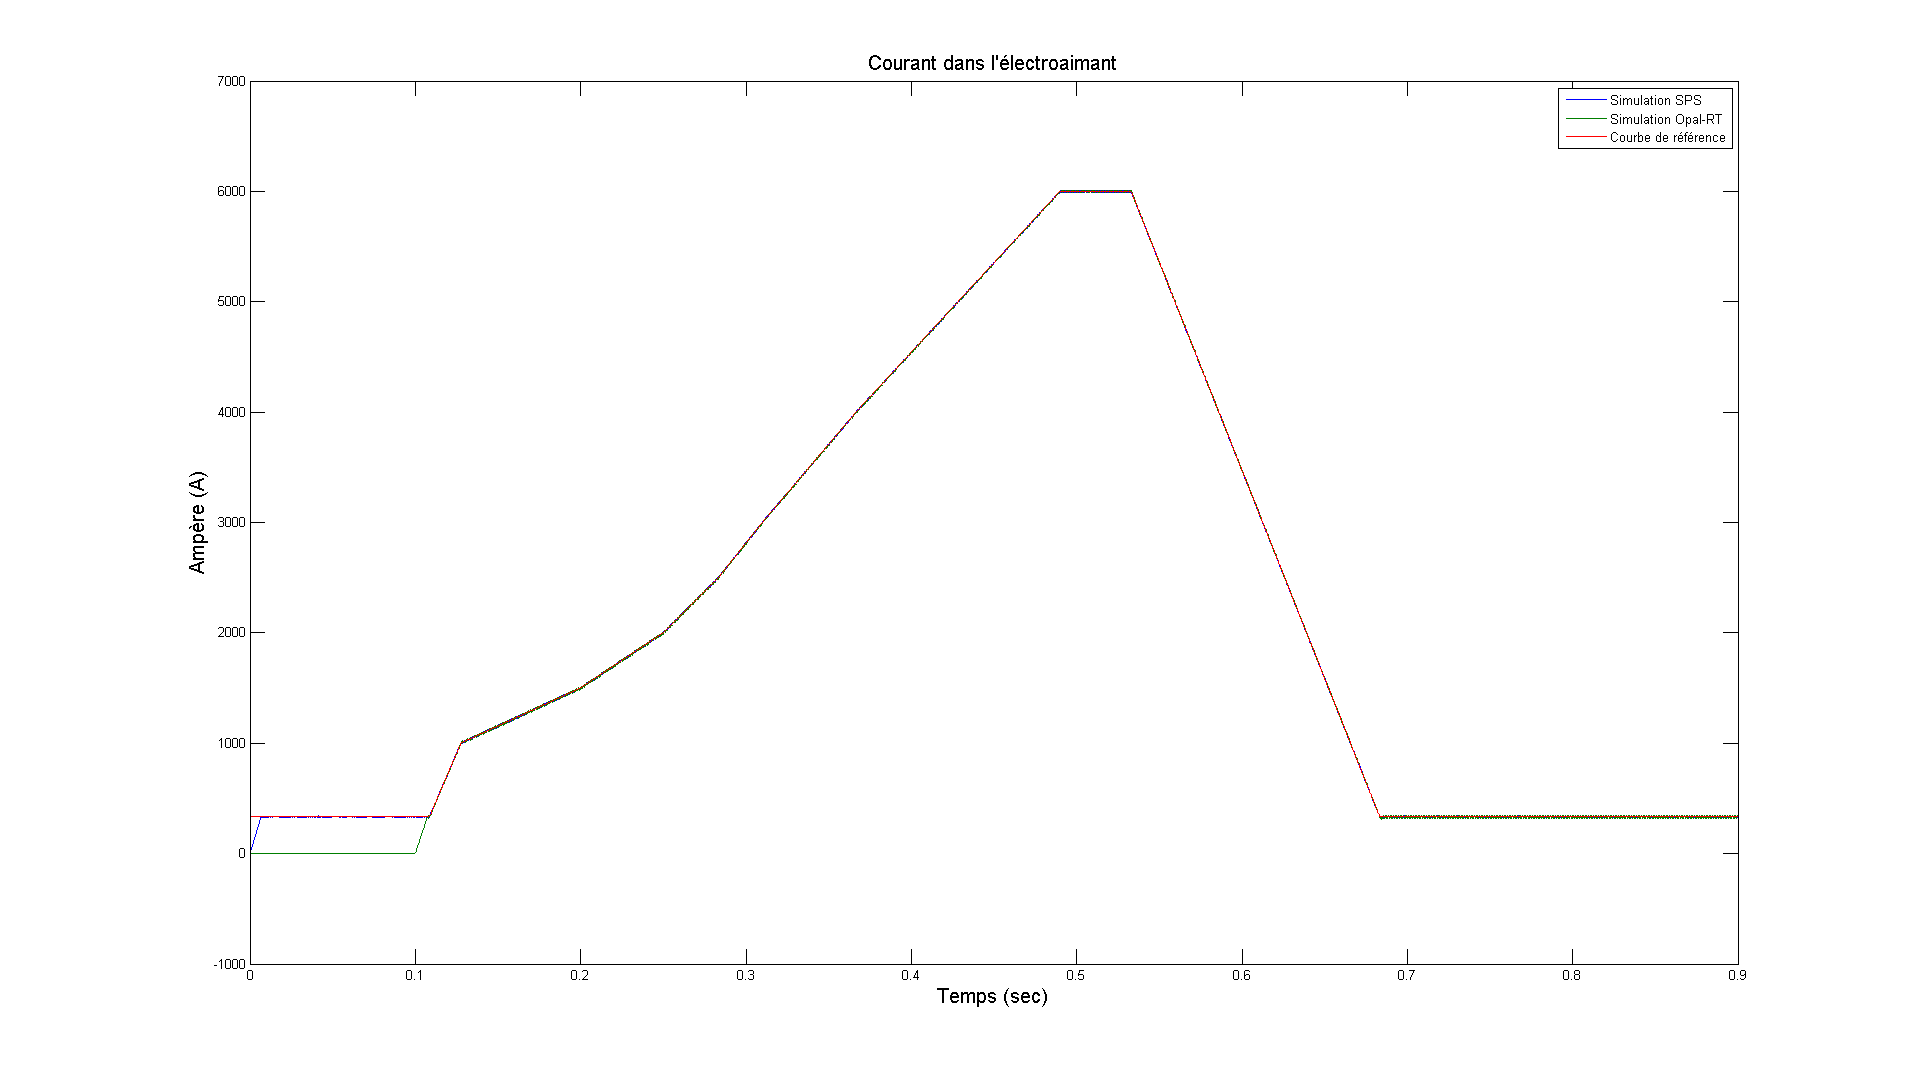
\includegraphics[scale=0.3]{fig/Opal-RT_Courant.png}}
\caption{Courant traversant la charge sur SPS et OPA4500}
\label{SPS_OPA4500_I_load}
\end{figure} 

\begin{figure}[htb]
\makebox[\textwidth][c]{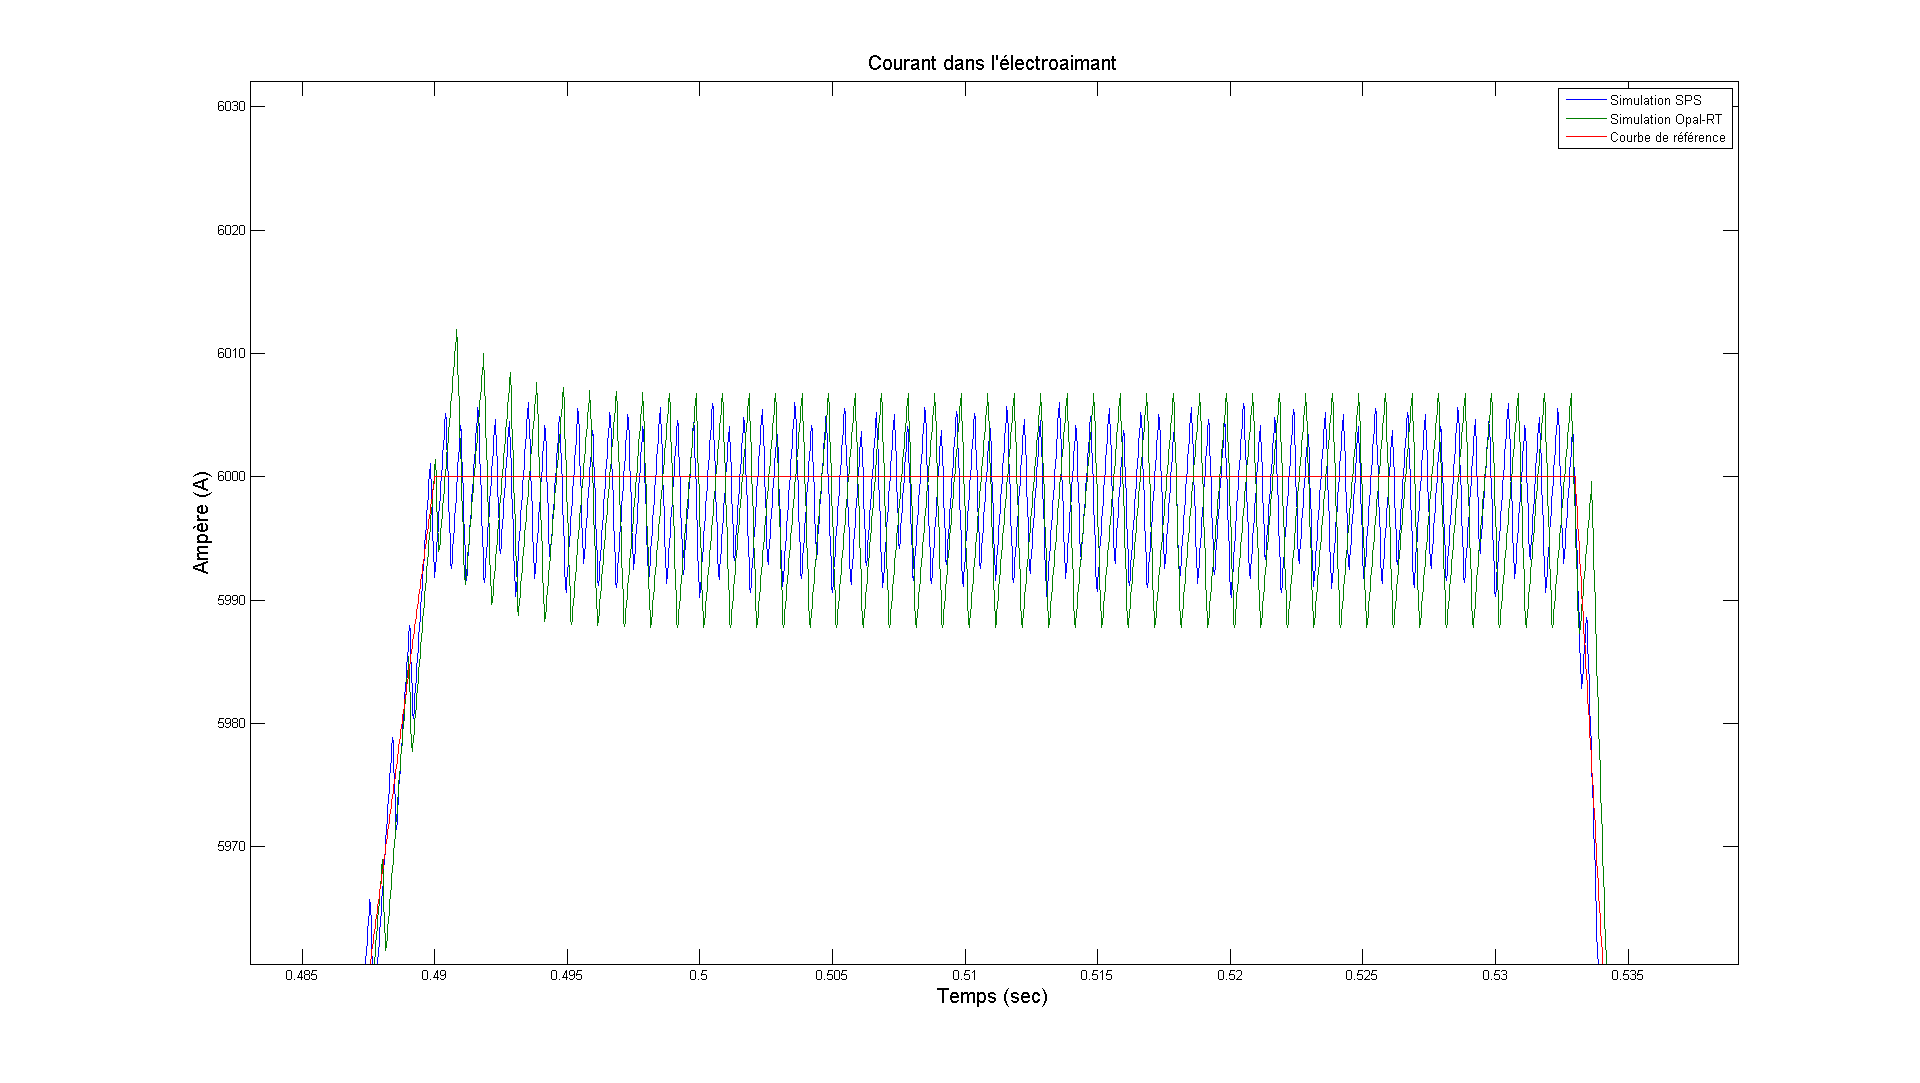
\includegraphics[scale=0.3]{fig/Opal-RT_Courant2.png}}
\caption{Courant traversant la charge ,sur la plage de maintien, sur SPS et OPA4500}
\label{SPS_OPA4500_I_load2}
\end{figure} 

\subsection{Analyse des résultats de simulation pour SPS et OPA4500}
La figure \ref{SPS_OPA4500_I_load} présente le courant traversant la charge sur l'ensemble d'un cycle dans le simulateur hors-ligne SPS et dans le simulateur temps réel OPA4500. Il est important de noter que pour un pas de 1$\mu$s dans SPS, le temps de simulation est de 1 minutes et 20 secondes sur SPS (AMD FX-8350 4 GHz) et de 0.9 secondes sur le simulateurs temps réel OPA-4500. On note évidemment que l'avantage en temps est substantiel. Il est cependant nécessaire de constater que les compromis du temps réel sont des estimations pessimistes des courants traversant la charge dans la période de maintien, comme on peut le voir à la figure \ref{SPS_OPA4500_I_load2}. Cependant, ces estimations, quoi que pessimistes, permettent une approximation très valable de la valeur attendue. Il est possible d'améliorer la précision de ces estimations en modifiant le paramètre $G_s$ qui correspond au paramètre de discrétisation dans Opal-RT. Ce paramètre régit la valeur de la résistance équivalente associée aux interrupteurs, aux composantes inductives et capacitives. Il permet de procéder à une solution de circuit purement réelle et ainsi, de minimiser la complexité de calcul. C'est grâce à ce genre d'approximation qu'il est possible d'obtenir du temps réel avec une simulation. Il est à noter que l'oscillation fournie par le simulateur temps réel OPA4500 est plus régulière que celle fournie dans le simulateur SPS. La représentation des composantes dans le OPA4500 fournie des résultats plus réguliers. Il est à noter que ce comportement n'est pas nécessairement plus réaliste.